\documentclass[aspectratio=169,11pt]{beamer}

% ── Packages ──────────────────────────────────────────────────────────────────
\usepackage{graphicx}
\usepackage{booktabs}
\usepackage{array}
\usepackage{xcolor}
\usepackage{tikz}
\usetikzlibrary{calc, positioning}
\usepackage{amsmath}
\usepackage{hyperref}
\usepackage{siunitx} % Added for better table alignment

% ── Colour Palette ────────────────────────────────────────────────────────────
\definecolor{DeepNavy}{HTML}{2E4057}
\definecolor{Teal}{HTML}{048A81}
\definecolor{WarmOrange}{HTML}{E85D04}
\definecolor{SoftPurple}{HTML}{9D4EDD}
\definecolor{WarmGray}{HTML}{8A8A8A}
\definecolor{LightGray}{HTML}{F2F2F2}
\definecolor{Cream}{HTML}{FFFDF7}
\definecolor{DeepRed}{HTML}{C1121F}
\definecolor{Gold}{HTML}{D4A017}

% ── Theme Setup ───────────────────────────────────────────────────────────────
\usetheme{default}
\setbeamertemplate{navigation symbols}{}
\setbeamertemplate{headline}{}
\setbeamercolor{background canvas}{bg=Cream}
\setbeamercolor{frametitle}{fg=DeepNavy,bg=Cream}
\setbeamerfont{frametitle}{series=\bfseries,size=\large}

\setbeamertemplate{frametitle}{%
  \vspace*{0.3em}%
  \insertframetitle%
  \ifx\insertframesubtitle\empty\else
    \\[0.1em]{\footnotesize\color{WarmGray}\insertframesubtitle}%
  \fi
  \vspace*{0.15em}%
  \textcolor{Teal}{\rule{\textwidth}{0.5pt}}%
}

\setbeamertemplate{footline}{%
  \hfill{\color{WarmGray}\tiny\insertframenumber\hspace{0.5em}}%
  \vspace{0.3em}%
}

\setbeamercolor{itemize item}{fg=Teal}
\setbeamercolor{itemize subitem}{fg=WarmOrange}
\setbeamertemplate{itemize item}{\small\raisebox{0.15ex}{\textbullet}}
\setbeamertemplate{itemize subitem}{\scriptsize\raisebox{0.15ex}{\textbullet}}

% ── Custom Macros ─────────────────────────────────────────────────────────────
\newcommand{\emphcolor}[1]{{\color{WarmOrange}\textbf{#1}}}
\newcommand{\tealtext}[1]{{\color{Teal}#1}}
\newcommand{\navytext}[1]{{\color{DeepNavy}#1}}
\newcommand{\graytext}[1]{{\color{WarmGray}#1}}

\newcommand{\transitionslide}[2]{%
  \begin{frame}[plain]
    \begin{tikzpicture}[remember picture, overlay]
      \fill[DeepNavy] (current page.south west) rectangle (current page.north east);
      \draw[Teal, opacity=0.3, line width=8pt] (current page.south west) ++(-1,-1)
        -- ++(20,0) -- ++(0,12) -- cycle;
      \node[text=white, font=\bfseries\LARGE, align=left, anchor=west] 
        at ($(current page.west)+(1.2,0.3)$) {#1};
      \node[text=Teal, font=\normalsize, align=left, anchor=west] 
        at ($(current page.west)+(1.2,-0.5)$) {#2};
    \end{tikzpicture}
  \end{frame}%
}

% ── Title frame ───────────────────────────────────────────────────────────────
\begin{document}

\begin{frame}[plain]
  \begin{tikzpicture}[remember picture, overlay]
    \fill[DeepNavy] (current page.south west) rectangle (current page.north east);
    \node[text=Teal, opacity=0.15, font=\fontsize{120}{120}\selectfont]
      at ($(current page.center)+(3,0)$) {\(\sim\)};
    % Shifted title up to avoid overlap with line [cite: 639]
    \node[text=white, font=\bfseries\fontsize{22}{26}\selectfont, align=left,
          anchor=west, text width=13cm]
      at ($(current page.west)+(1.0,1.5)$)
      {Climate Shocks, Health Finance,\\and Economic Outcomes};
    \node[text=Teal, font=\normalsize, align=left, anchor=west]
      at ($(current page.west)+(1.0,0.1)$)
      {County-Level Evidence from the United States, 2011--2023};
    \node[text=WarmGray, font=\small, align=left, anchor=west]
      at ($(current page.west)+(1.0,-0.7)$)
      {Thesis Committee Update \(\cdot\) March 2026};
    % Shifted line down to create clear separation [cite: 642]
    \draw[WarmOrange, line width=2pt]
      ($(current page.west)+(1.0,0.5)$) -- ++(11,0);
  \end{tikzpicture}
\end{frame}

% ── Main Cold Results ─────────────────────────────────────────────────────────
\begin{frame}{Extreme Cold Raises Premiums, Bad Debt, and Medical Debt}
  \framesubtitle{Local Projections, $h=0$, state-clustered SEs [cite: 270]}
  \begin{center}
    \small
    \begin{tabular}{lrrl}
      \toprule
      \textbf{Outcome} & \textbf{Estimate} & \textbf{(SE)} & \textbf{Significance} \\
      \midrule
      Benchmark Silver Premium & $+\$30.67$ & $(9.92)$ & \emphcolor{***} [cite: 272, 668] \\
      Hospital Bad Debt per Capita & $+\$4.43$ & $(1.60)$ & \emphcolor{***} [cite: 272, 668] \\
      Medical Debt Share & $+0.29$ pp & $(0.15)$ & \emphcolor{*} [cite: 272, 669] \\
      \midrule
      Median HH Income & $+\$103$ & $(74)$ & \graytext{n.s.} [cite: 272, 669] \\
      Per Capita Income & $-\$107$ & $(268)$ & \graytext{n.s.} [cite: 272, 669] \\
      Civilian Employment & $-269$ & $(199)$ & \graytext{n.s.} [cite: 272, 669] \\
      \bottomrule
    \end{tabular}
  \end{center}
  \vspace{0.3em}
  \begin{columns}[T]
    \begin{column}{0.48\textwidth}
      \emphcolor{\$30.67 premium increase} = \emphcolor{7\%} of avg plan [cite: 273, 459]\\
      \graytext{\footnotesize Comparable to tobacco surcharge (5--15\%) [cite: 274]}
    \end{column}
    \begin{column}{0.48\textwidth}
      \emphcolor{+\$4.43/capita} = \emphcolor{\$443k per 100k county} [cite: 275, 469]\\
      \graytext{\footnotesize Non-trivial hospital balance-sheet hit [cite: 276]}
    \end{column}
  \end{columns}
\end{frame}

% ── The Heat Paradox Slide ────────────────────────────────────────────────────
\begin{frame}{Extreme Heat Hits Household Income, Not Health Costs}
  \framesubtitle{Local Projections, $h=0$ [cite: 330]}
  \begin{columns}[T]
    \begin{column}{0.62\textwidth}
      \includegraphics[width=\textwidth]{../Analysis/plots/event_study/lp_High_CDD_Med_HH_Income_Real.png}
    \end{column}
    \begin{column}{0.34\textwidth}
      \small
      \begin{tabular}{lrl}
        \toprule
        \textbf{Outcome} & \textbf{Est.} & \\
        \midrule
        Med. HH Income & \emphcolor{$-\$265^{***}$} & [cite: 342, 676] \\
        Silver Premium & $-\$2.4$ & \graytext{n.s.} [cite: 342, 676] \\
        Medical Debt & $-0.32$ pp & \graytext{n.s.} [cite: 342, 676] \\
        Hosp. Bad Debt & $+\$2.3$ & \graytext{n.s.} [cite: 342, 676] \\
        \bottomrule
      \end{tabular}
      \vspace{0.8em}
      \textbf{Possible mechanisms:} [cite: 343]
      \begin{itemize}
        \item Labour supply disruption [cite: 344]
        \item AC energy costs [cite: 345]
        \item Outdoor/agricultural loss [cite: 346]
      \end{itemize}
      \tealtext{Health costs unaffected: ubiquitous AC? [cite: 347]}
    \end{column}
  \end{columns}
\end{frame}

% ── Corrected Asymmetry TikZ Slide ────────────────────────────────────────────
\begin{frame}{Cold vs.\ Heat: A Clear Asymmetry}
  \begin{center}
    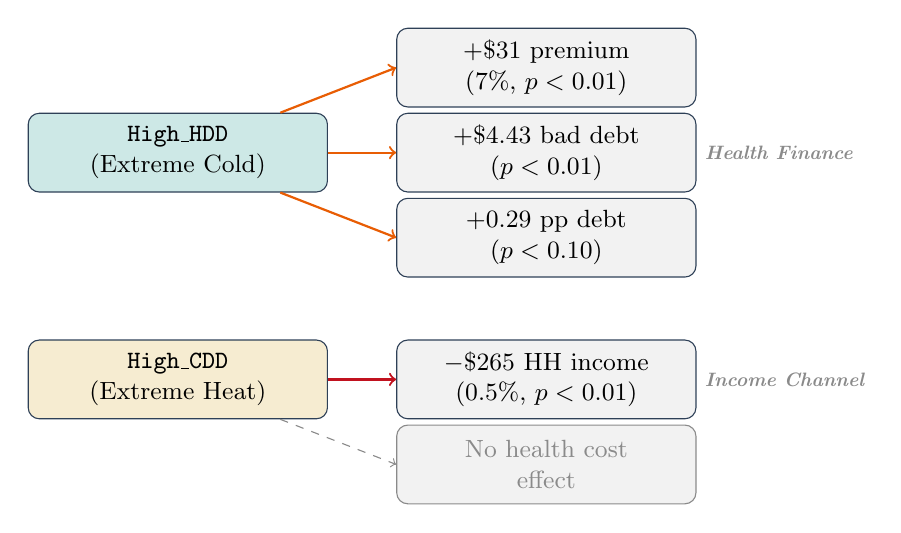
\begin{tikzpicture}[scale=0.9,
      box/.style={draw=DeepNavy, rounded corners=4pt, fill=LightGray, 
                  minimum width=3.8cm, minimum height=1.0cm, align=center, font=\small}]
      % Causes - Shifted slightly for spacing [cite: 678, 681]
      \node[box, fill=Teal!20] (cold) at (0,0) {\texttt{High\_HDD}\\(Extreme Cold)};
      \node[box, fill=Gold!20] (heat) at (0,-3.2) {\texttt{High\_CDD}\\(Extreme Heat)};

      % Outcomes - Corrected alignment and padding [cite: 679, 680, 682]
      \node[box] (prem) at (5.2, 1.2)  {$+\$31$ premium\\(7\%, $p<0.01$)};
      \node[box] (bad)  at (5.2, 0.0)  {$+\$4.43$ bad debt\\($p<0.01$)};
      \node[box] (debt) at (5.2,-1.2) {$+0.29$ pp debt\\($p<0.10$)};
      \node[box] (inc)  at (5.2,-3.2) {$-\$265$ HH income\\(0.5\%, $p<0.01$)};
      \node[box, draw=WarmGray, text=WarmGray] (none) at (5.2,-4.4) {No health cost\\effect};

      % Arrows
      \draw[->, WarmOrange, thick] (cold) -- (prem.west);
      \draw[->, WarmOrange, thick] (cold) -- (bad.west);
      \draw[->, WarmOrange, thick] (cold) -- (debt.west);
      \draw[->, DeepRed, thick] (heat) -- (inc.west);
      \draw[->, WarmGray, dashed] (heat) -- (none.west);

      % Channel Labels [cite: 684]
      \node[font=\scriptsize\itshape\bfseries, text=WarmGray, anchor=west] at (7.3, 0.0) {Health Finance};
      \node[font=\scriptsize\itshape\bfseries, text=WarmGray, anchor=west] at (7.3,-3.2) {Income Channel};
    \end{tikzpicture}
  \end{center}
  \vspace{0.2em}
  \begin{center}
    \tealtext{This asymmetry is a novel contribution to the climate-health literature [cite: 360]}
  \end{center}
\end{frame}

\end{document}